\chapter{IPv6: Part 2}\label{ipv6-part-2}

IPv6 ADDRESS CONFIGURATION (EUI-64)

\begin{itemize}
\tightlist
\item
  EUI stands for Extended Unique Identifier
\item
  (Modified) EUI-64 is a method of converting a MAC address (48-bits)
  into a 64-bit INTERFACE identifier
\item
  This INTERFACE identifier can then become the ``HOST portion'' of a
  /64 IPv6 ADDRESS
\end{itemize}

\begin{figure}
\centering
\pandocbounded{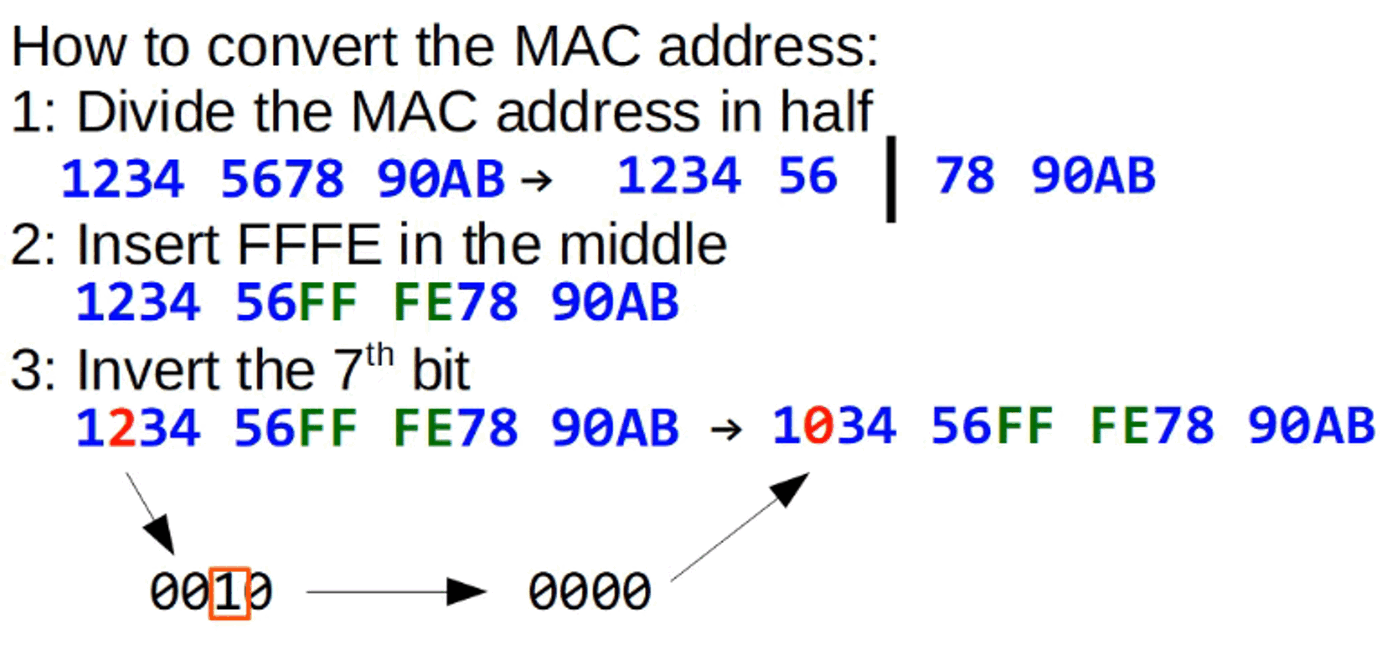
\includegraphics[keepaspectratio,alt={image}]{images/33-ipv6-part2/img-001.png}}
\end{figure}

EUI-64 PRACTICE:

\begin{lstlisting}
782B CBAC 0867 >>> 782B CB  ||  AC 0867

782B CBFF  FEAC 0867

8 is the 7th bit so 1000 inverted becomes 1010 = A in hex

so the EUI-64 Interface Identifier is :  7A2B CBFF FEAC 0867
\end{lstlisting}

\begin{figure}
\centering
\pandocbounded{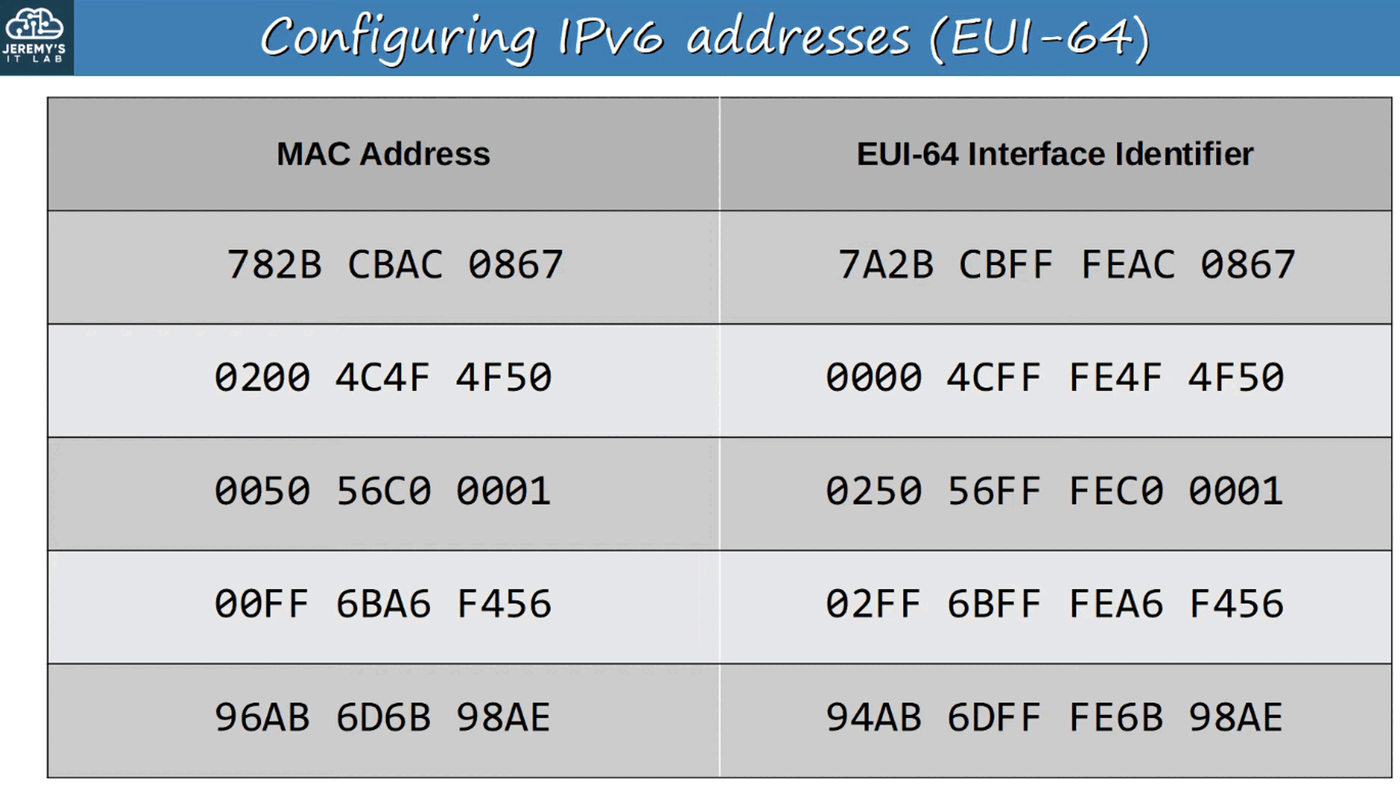
\includegraphics[keepaspectratio,alt={image}]{images/33-ipv6-part2/img-002.png}}
\end{figure}

CONFIGURING IPv6 ADDRESSES with EUI-64

\begin{figure}
\centering
\pandocbounded{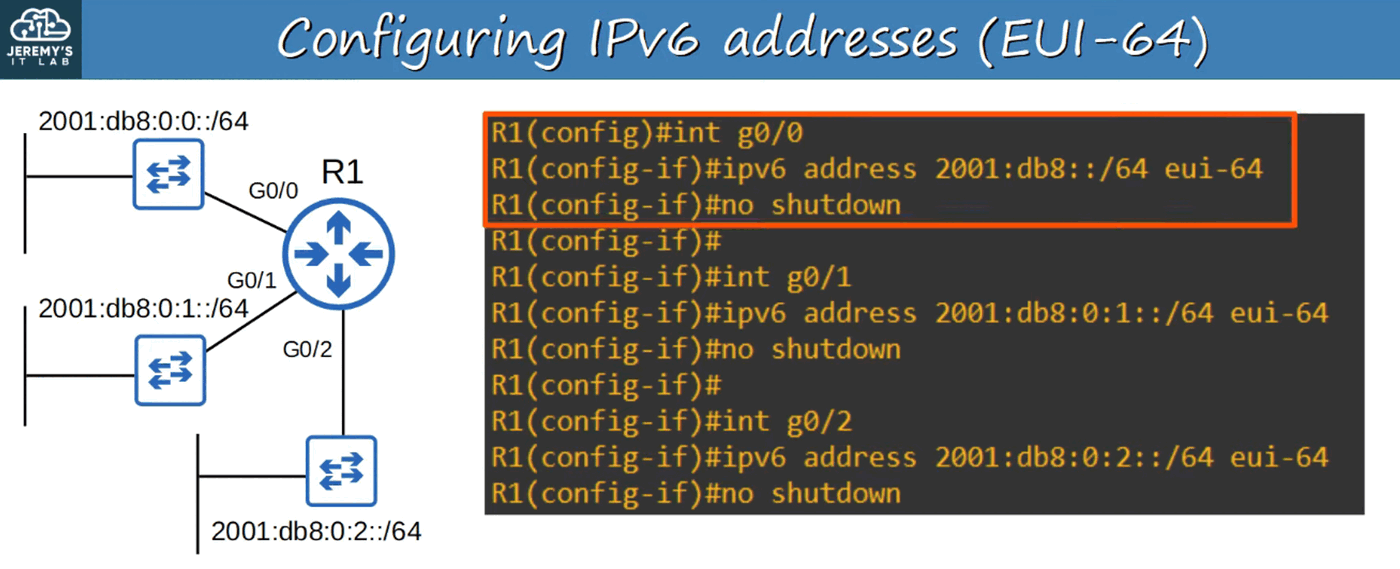
\includegraphics[keepaspectratio,alt={image}]{images/33-ipv6-part2/img-003.png}}
\end{figure}

\begin{figure}
\centering
\pandocbounded{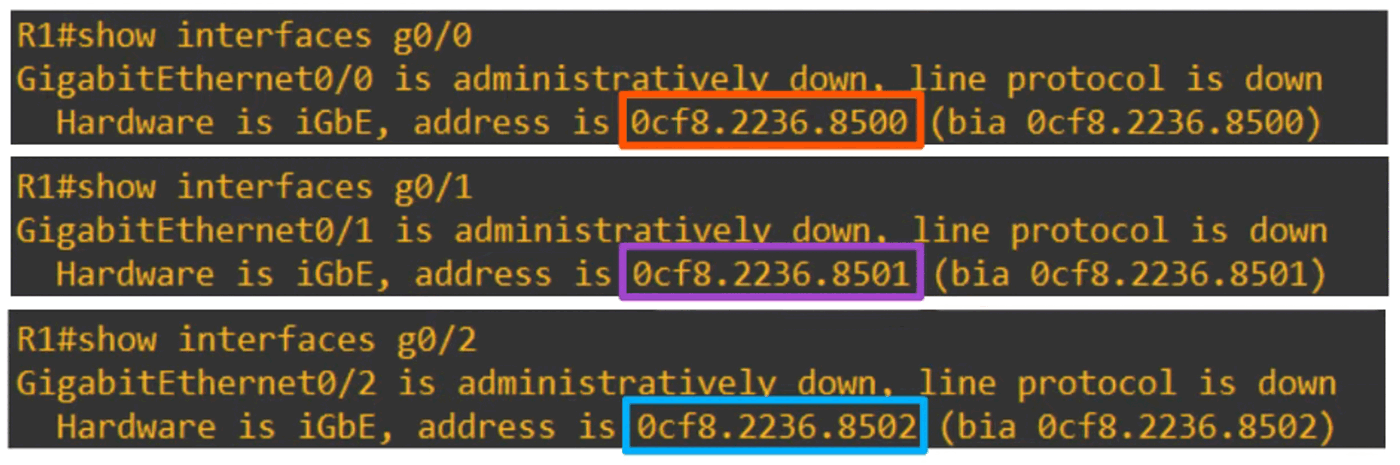
\includegraphics[keepaspectratio,alt={image}]{images/33-ipv6-part2/img-004.png}}
\end{figure}

\begin{figure}
\centering
\pandocbounded{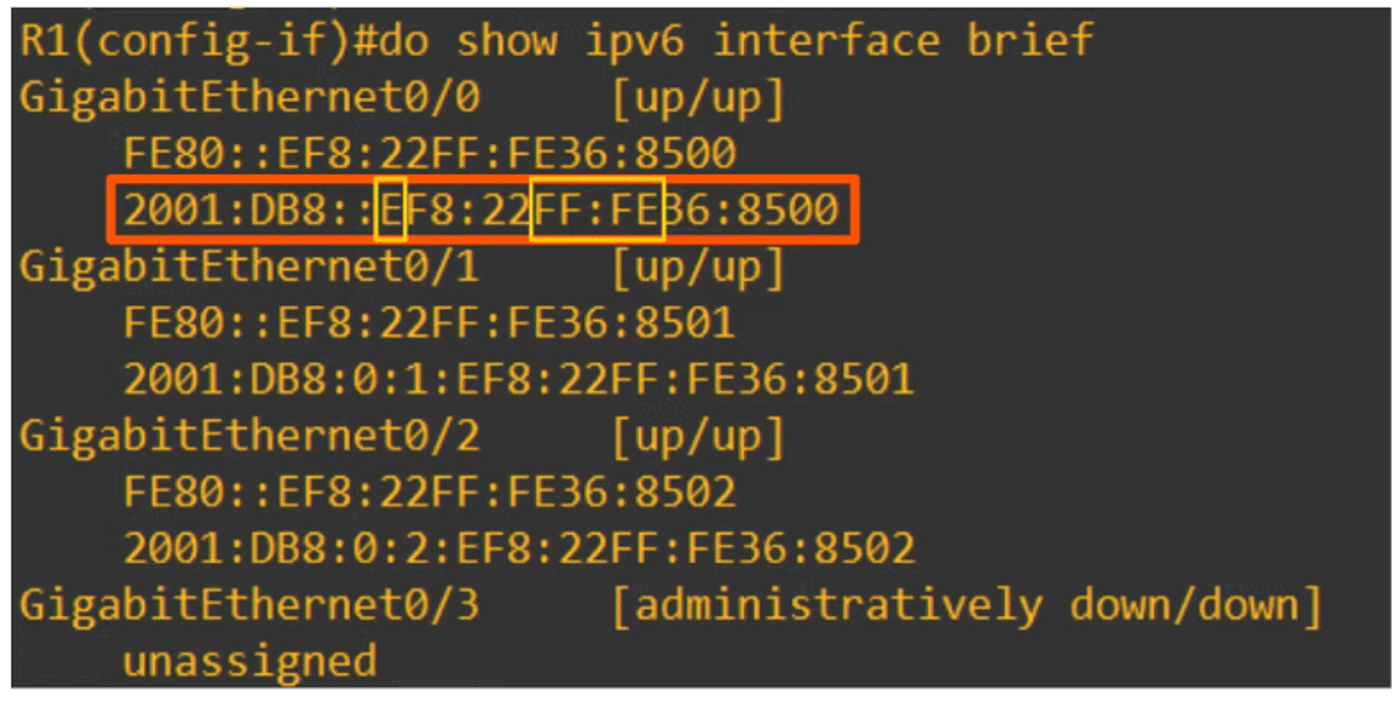
\includegraphics[keepaspectratio,alt={image}]{images/33-ipv6-part2/img-005.png}}
\end{figure}

NOTE the ``2001:DB8\ldots'' Address has ``E'' changed to ``c''. This is
the 7th bit getting flipped (1110 to 1100 = 12 = hex `C')

WHY INVERT THE 7th BIT ?

\begin{itemize}
\tightlist
\item
  MAC addresses can be divided into TWO TYPES:

  \begin{itemize}
  \tightlist
  \item
    UAA (Universally Administered Address)

    \begin{itemize}
    \tightlist
    \item
      Uniquely assigned to the device of the manufacturer
    \end{itemize}
  \item
    LAA (Locally Administered Address)

    \begin{itemize}
    \tightlist
    \item
      Manually assigned by an Admin (with the mac-address command on the
      INTERFACE) or protocol. Doesn't have to be globally unique.
    \end{itemize}
  \end{itemize}
\item
  You can INDENTIFY a UAA or LAA by the 7th bit of the MAC ADDRESS,
  called the U/L bit (Universal/Local bit)

  \begin{itemize}
  \tightlist
  \item
    U/L bit set to 0 = UAA
  \item
    U/L bit set to 1 = LAA
  \end{itemize}
\item
  In the context of IPv6 addresses/EUI-64, the meaning of the U/L bit is
  reversed:

  \begin{itemize}
  \tightlist
  \item
    U/L bit set to 0 = The MAC address the EUI-64 INTERFACE ID was made
    from was an LAA
  \item
    U/L bit set to 1 = The MAC address the EUI-64 INTERFACE ID was made
    from was a UAA
  \end{itemize}
\end{itemize}

IPv6 ADDRESS TYPES

\begin{enumerate}
\def\labelenumi{\arabic{enumi})}
\tightlist
\item
  GLOBAL UNICAST ADDRESSES
\end{enumerate}

\begin{itemize}
\tightlist
\item
  \textbf{Global Unicast} IPv6 ADDRESSES are PUBLIC ADDRESSES which can
  be used over the INTERNET
\item
  Must REGISTER to use them.
\item
  They are PUBLIC ADDRESSES so need to be GLOBALLY UNIQUE
\end{itemize}

Originally defined as the 2000 :: /3 block (2000:: to 3FFF : FFFF : FFFF
: FFFF : FFFF : FFFF : FFFF : FFFF)

\begin{itemize}
\tightlist
\item
  NOW defined as ALL ADDRESSES which are not RESERVED for other purposes
\end{itemize}

Remember THESE THREE PARTS of a GLOBAL UNICAST ADDRESS

\begin{figure}
\centering
\pandocbounded{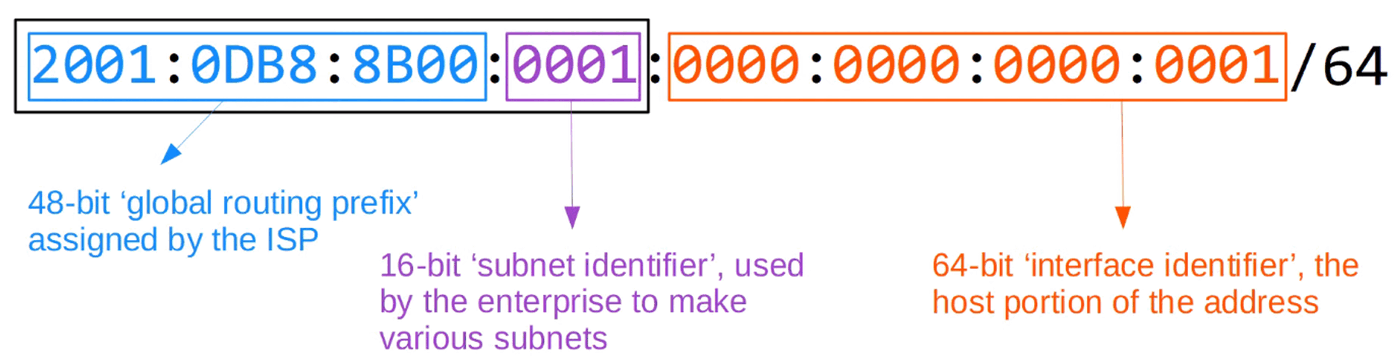
\includegraphics[keepaspectratio,alt={image}]{images/33-ipv6-part2/img-006.png}}
\end{figure}

\begin{enumerate}
\def\labelenumi{\arabic{enumi})}
\setcounter{enumi}{1}
\tightlist
\item
  UNIQUE LOCAL ADDRESSES
\end{enumerate}

\begin{itemize}
\tightlist
\item
  \textbf{Unique Local} IPv6 ADDRESSES are PRIVATE ADDRESSES which
  cannot be used over the internet
\item
  You do NOT need to REGISTER to use them
\item
  Can be used FREELY within INTERNAL NETWORKS
\item
  Do NOT need to be GLOBALLY UNIQUE (*)
\item
  CANNOT be ROUTED over the INTERNET
\end{itemize}

\begin{tipbox}

Uses the ADDRESS block FC00 ::/7 (FC00:: to FDFF : FFFF : FFFF : FFFF :
FFFF : FFFF : FFFF : FFFF)

\end{tipbox}

\begin{itemize}
\tightlist
\item
  A later UPDATE required the 8th bit to be set to 1 so the FIRST TWO
  DIGITS must be FD
\end{itemize}

(*) The GLOBAL ID should be UNIQUE so that ADDRESSES don't overlap when
companies MERGE

\begin{figure}
\centering
\pandocbounded{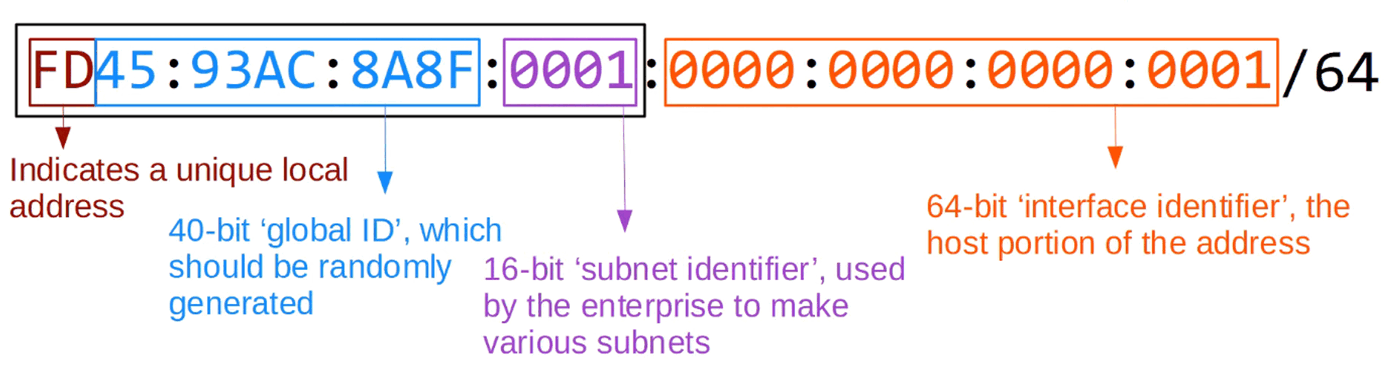
\includegraphics[keepaspectratio,alt={image}]{images/33-ipv6-part2/img-007.png}}
\end{figure}

\begin{enumerate}
\def\labelenumi{\arabic{enumi})}
\setcounter{enumi}{2}
\tightlist
\item
  LINK-LOCAL ADDRESSES
\end{enumerate}

\begin{itemize}
\tightlist
\item
  \textbf{Link-Local} IPv6 ADDRESSES are AUTOMATICALLY generated on
  IPv6-enabled INTERFACES
\item
  Use command \passthrough{\lstinline!R1(config-if)\# ipv6 enable!} on
  an interface to enable IPv6 on an INTERFACE
\end{itemize}

\begin{tipbox}

Uses the ADDRESS block FE80::/10 (FE80:: to FEBF : FFFF : FFFF : FFFF :
FFFF : FFFF : FFFF : FFFF)

\end{tipbox}

\begin{itemize}
\tightlist
\item
  The STANDARD states that the 54-bits AFTER FE80/10 should be ALL 0's
  so you won't see Link-Local ADDRESSES beginning with FE9, FEA, or FEB
  - ONLY FE8(!)
\item
  The INTERFACE ID is generated using EUI-64 rules
\item
  Link-Local means that these addresses are used for communication
  within a single link (SUBNET)

  \begin{itemize}
  \tightlist
  \item
    ROUTER will not route PACKETS with a Link-Local DESTINATION IPv6
    ADDRESS
  \end{itemize}
\item
  Common uses of Link-Local Addresses:

  \begin{itemize}
  \tightlist
  \item
    Routing Protocol Peerings (OSPFv3 uses Link-Local Addresses for
    Neighbour Adjacencies)
  \item
    NEXT-HOP ADDRESS for STATIC ROUTES
  \item
    Neighbor Discovery Protocol (NDP, IPv6's replacement for ARP) uses
    Link-Local ADDRESSES to function
  \end{itemize}

  Network using Link-Local Addresses for ``next-hop'' routing
\end{itemize}

\begin{figure}
\centering
\pandocbounded{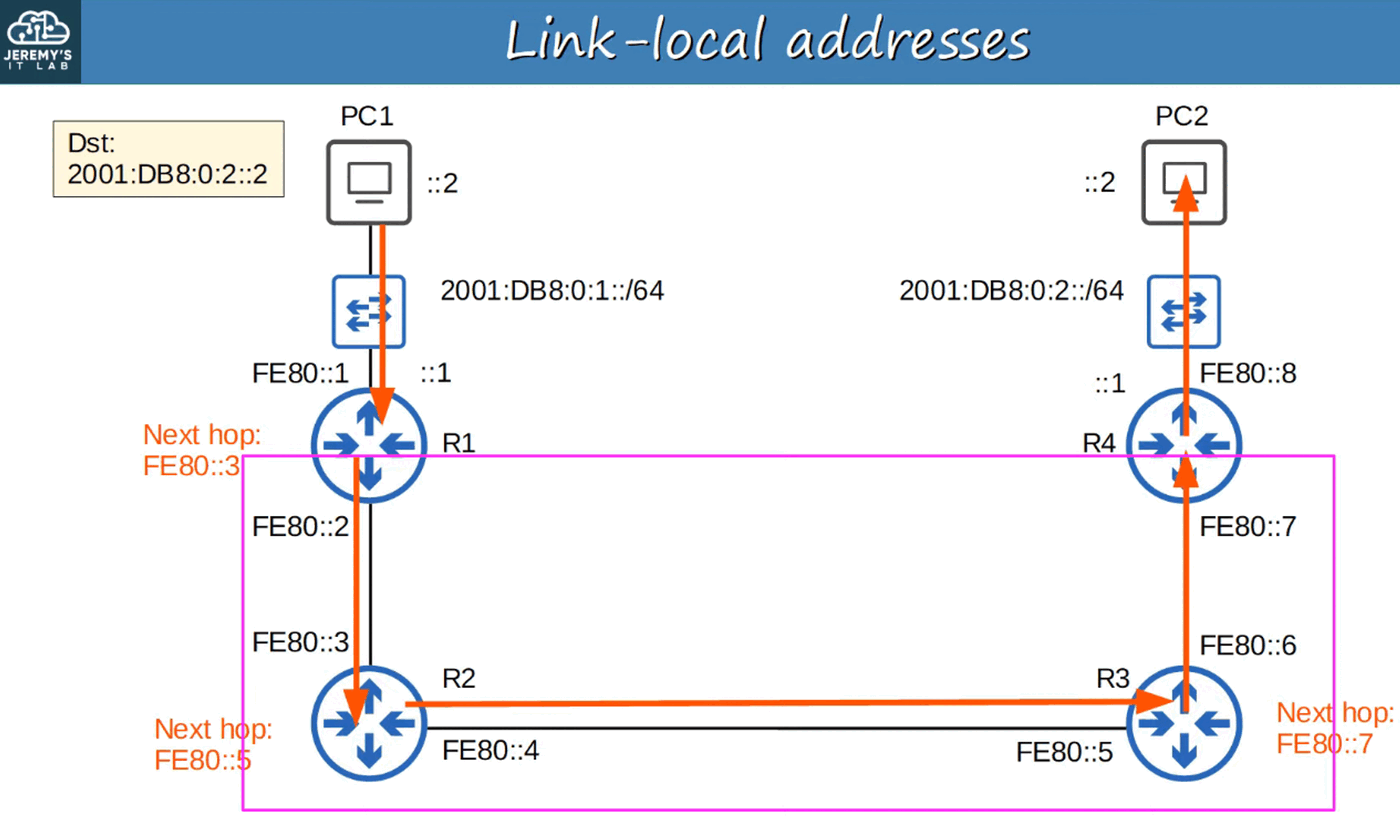
\includegraphics[keepaspectratio,alt={image}]{images/33-ipv6-part2/img-008.png}}
\end{figure}

\begin{enumerate}
\def\labelenumi{\arabic{enumi})}
\setcounter{enumi}{3}
\tightlist
\item
  MULTICAST ADDRESSES
\end{enumerate}

\begin{itemize}
\tightlist
\item
  \textbf{Unicast Addresses} are one-to-one

  \begin{itemize}
  \tightlist
  \item
    ONE SOURCE to ONE DESTINATION
  \end{itemize}
\item
  \textbf{\emph{Broadcast}} Addresses are one-to-all

  \begin{itemize}
  \tightlist
  \item
    ONE SOURCE to ALL DESTINATIONS (within the subnet)
  \end{itemize}
\item
  \textbf{Multicast} Addresses are one-to-many

  \begin{itemize}
  \tightlist
  \item
    ONE SOURCE to MULTIPLE DESTINATIONS (that have joined the specific
    \textbf{\emph{multicast}} group)
  \end{itemize}
\end{itemize}

\begin{tipbox}

IPv6 uses range FF00::/8 for multicast (FF00:: to FFFF : FFFF : FFFF :
FFFF : FFFF : FFFF : FFFF : FFFF)

\end{tipbox}

\begin{itemize}
\tightlist
\item
  \textbf{IPv6 doesn't use Broadcast} (there IS NO ``Broadcast Address''
  in IPv6!)
\end{itemize}

\section{You Must Know the Multicast Address for Each Router
Type}\label{you-must-know-the-multicast-address-for-each-router-type}

NOTE that the IPv6 and IPv4 Addresses share the same last digit

\begin{figure}
\centering
\pandocbounded{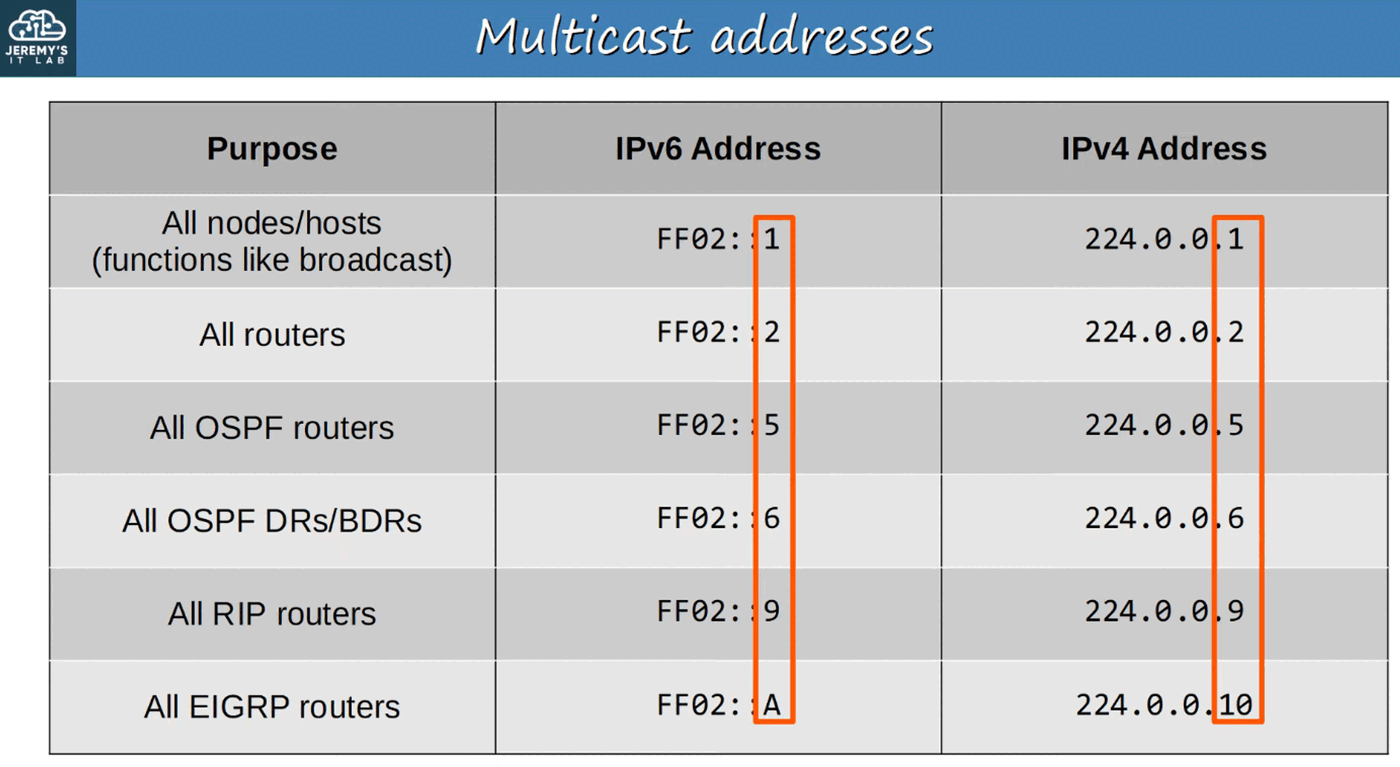
\includegraphics[keepaspectratio,alt={image}]{images/33-ipv6-part2/img-009.png}}
\end{figure}

\section{Multicast Address Scopes}\label{multicast-address-scopes}

\begin{itemize}
\tightlist
\item
  IPv6 defines multiple MULTICAST `scopes' which indicate how far the
  PACKET should be forwarded
\item
  The ADDRESS in the previous slide all use the `link-local' scope
  (FF02), which stays in the LOCAL SUBNET
\end{itemize}

\textbf{IPv6 Multicast Scope Types:}

\begin{itemize}
\tightlist
\item
  \textbf{Interface-Local (FF01)}

  \begin{itemize}
  \tightlist
  \item
    The PACKET doesn't leave the LOCAL device
  \item
    Can be used to SEND traffic to a SERVICE within the LOCAL device
  \end{itemize}
\item
  \textbf{Link-Local (FF02)}

  \begin{itemize}
  \tightlist
  \item
    The PACKET remains in the LOCAL SUBNET
  \item
    ROUTERS will not route the PACKET between SUBNETS
  \end{itemize}
\item
  \textbf{Site-Local (FF05)}

  \begin{itemize}
  \tightlist
  \item
    The PACKET can be forwarded by ROUTERS
  \item
    Should be limited to a SINGLE PHYSICAL LOCATION (not forwarded over
    a WAN)
  \end{itemize}
\item
  \textbf{Organization-Local (FF08)}

  \begin{itemize}
  \tightlist
  \item
    Wider in scope than Site-Local (an entire company / ORGANIZATION)
  \end{itemize}
\item
  \textbf{Global (FF0E)}

  \begin{itemize}
  \tightlist
  \item
    No boundaries
  \item
    Possible to be ROUTED over the INTERNET
  \end{itemize}
\end{itemize}

\begin{figure}
\centering
\pandocbounded{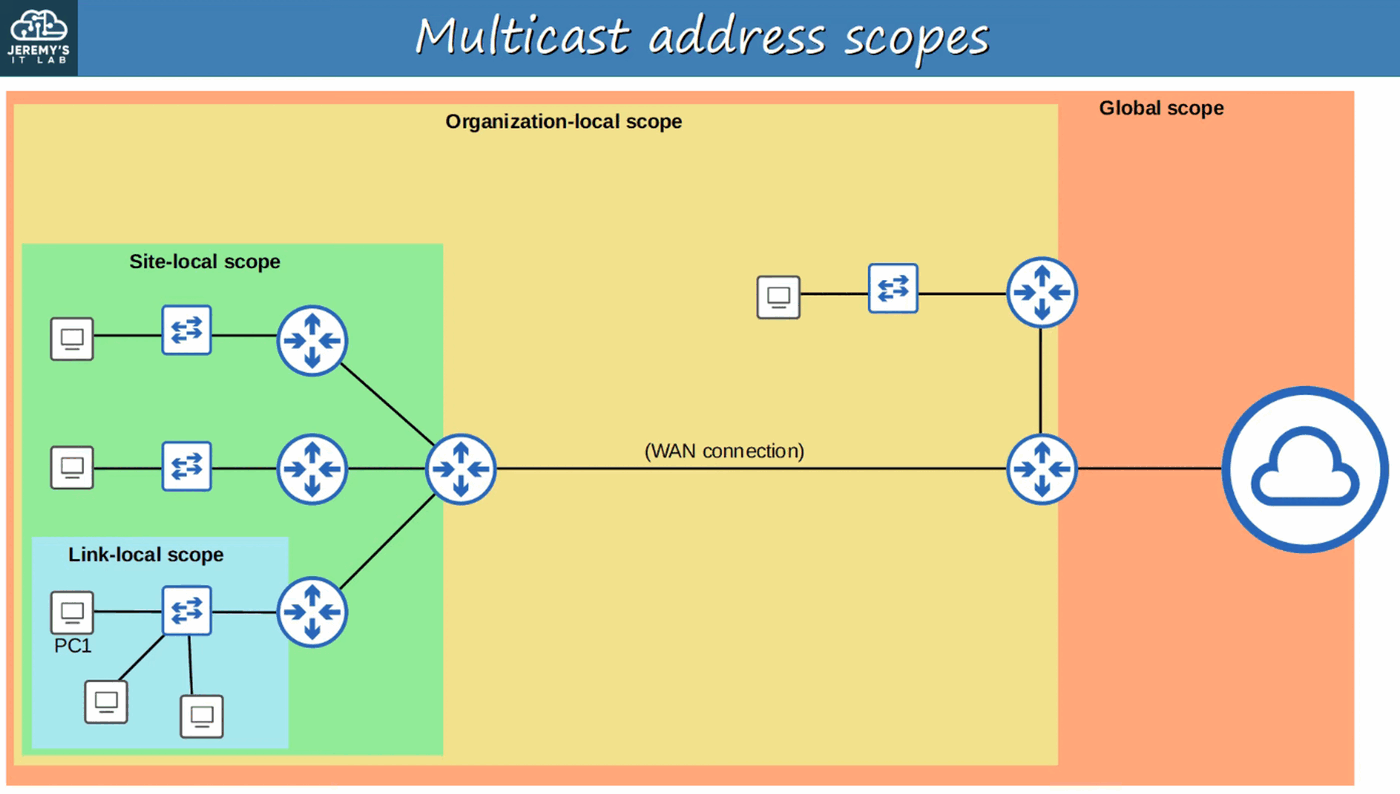
\includegraphics[keepaspectratio,alt={image}]{images/33-ipv6-part2/img-010.png}}
\end{figure}

\begin{enumerate}
\def\labelenumi{\arabic{enumi})}
\setcounter{enumi}{4}
\tightlist
\item
  ANYCAST ADDRESS
\end{enumerate}

\begin{itemize}
\tightlist
\item
  \textbf{ANYCAST is a NEW feature of IPv6}
\item
  ANYCAST is `one-to-one-of-many'
\item
  Multiple ROUTERS are configured with the SAME IPv6 ADDRESS

  \begin{itemize}
  \tightlist
  \item
    They use a ROUTING PROTOCOL to advertise the address
  \item
    When HOSTS sends PACKETS to that DESTINATION ADDRESS, ROUTERS will
    forward it to the NEAREST ROUTER configured with THAT IP ADDRESS
    (based on ROUTING METRIC)
  \end{itemize}
\item
  There is NO SPECIFIC ADDRESS range for ANYCAST ADDRESSES.

  \begin{itemize}
  \tightlist
  \item
    Use a regular UNICAST (Global Unicast, Unique Local) and specify
    THAT as an ANYCAST ADDRESS
  \item
    \passthrough{\lstinline!R1(config-if)\# ipv6 address 2000:db8:1:1::99/128 anycast!}
  \end{itemize}
\end{itemize}

\begin{figure}
\centering
\pandocbounded{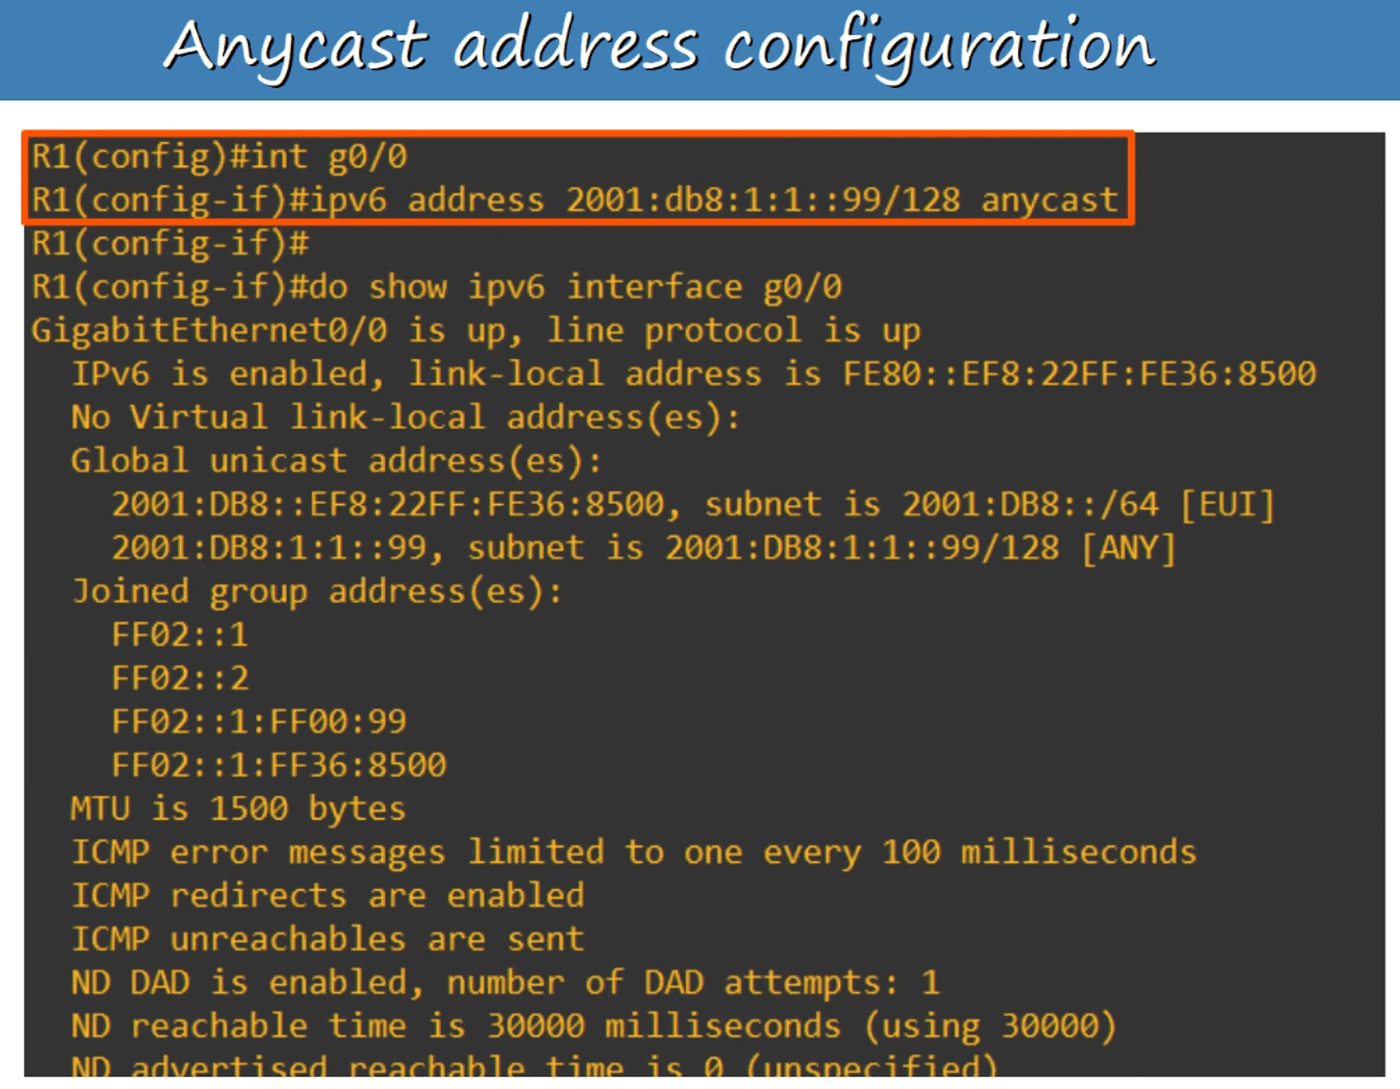
\includegraphics[keepaspectratio,alt={image}]{images/33-ipv6-part2/img-011.png}}
\end{figure}

\begin{enumerate}
\def\labelenumi{\arabic{enumi})}
\setcounter{enumi}{5}
\tightlist
\item
  OTHER IPv6 ADDRESSES
\end{enumerate}

\begin{itemize}
\tightlist
\item
  The :: Address = The \emph{unspecified} IPv6 ADDRESS

  \begin{itemize}
  \tightlist
  \item
    Can be used when a DEVICE doesn't yet know its IPv6 ADDRESS
  \item
    IPv6 DEFAULT ROUTES are configured to ::/0
  \item
    IPv4 equivalent: 0.0.0.0
  \end{itemize}
\item
  The ::1 Address = The Loopback Address

  \begin{itemize}
  \tightlist
  \item
    Used to test the PROTOCOL STACK on the LOCAL DEVICE
  \item
    Messages sent to THIS ADDRESS are processed within the LOCAL DEVICE
    but not SENT to other DEVICES
  \item
    IPv4 equivalent : 127.0.0.0 /8 address range
  \end{itemize}
\end{itemize}
